

\chapter{Ataques a redes neuronales} % Main chapter title

\label{Ataques} % Change X to a consecutive number; for referencing this chapter elsewhere, use \ref{ChapterX}

%----------------------------------------------------------------------------------------
%	SECTION 1
%----------------------------------------------------------------------------------------
La seguridad de los sistemas de aprendizaje automático es vulnerable y sus ataques son conocidos en la literatura como ataques adversarios [adversarial attack] en el cual intencionalmente el atacante intenta alterar la respuesta de un clasificador, ya sea interviniendo el proceso de entrenamiento o bien el proceso de validación u operación. Por ejemplo, puede producir una pequeña perturbación en los datos de entrada \parencite{r49} que llevaría al clasificador entregar un resultado erróneo aun cuando esta perturbación puede resultar imperceptible al ojo humano \parencite{r4}, pero suficiente para que el clasificador arroje una salida errónea o una deseada por el atacante. Lo anterior se puede evidenciar en:
\begin{itemize}

\item En el caso de la visión artificial, en donde existen estudios en los que se simula un ataque a un clasificador de señaléticas de tránsito de vehículos con conducción automática \parencite{r8} para que sean interpretadas de manera errónea por sus sistemas, siendo esta modificación imperceptible para un conductor humano. También se ha llegado a crear ataques físicos, en los cuales la perturbación se lleva a cabo en el mundo físico, en el cual los ataques adversarios también toman efecto \parencite{r12}. 

\item En el caso de los intérpretes de voz como Amazon Alexa o Google Home, donde se han hecho estudios en los cuales dichos sistemas son atacados mediante ultrasonido o ruidos de fondo ocultos \parencite{r17}, e incluso en mensajes que parecen auténticos o canciones \parencite{r31} que poseen comandos de voz ocultos no perceptible por personas.
    
\end{itemize}
En los años recientes varios estudios han demostrado distintas técnicas que provocan fallos en el proceso de clasificación de una red neuronal artificial. Esto ha impuesto el concepto de robustez, el cual señala que tan segura es una red frente a los tipos de ataque que puede recibir. Los ataques adversarios se clasifican en dos grupos, el primero es el llamado “ataque de caja blanca” \parencite{r19} en donde el atacante tiene completo conocimiento sobre el modelo de la red, incluido la topología, entradas, salidas y pesos de sus conexiones. En el segundo llamado “ataque de caja negra” se asume que el atacante sólo tiene acceso a la entrada y salida del modelo, y no sabe nada sobre su topología, pesos de sus conexiones. 
A continuación, se presentan los principales tipos de ataques:




\section{Ataque de extracción de modelo}

El objetivo principal del ataque de extracción de modelo (Model extraction attack) es robar la propiedad intelectual del modelo sin conocimiento previo de los datos y algoritmos de entrenamiento. También podría ser utilizado para ejecutar un ataque de caja negra, siendo usado como modelo sustituto, explotando la capacidad de los ejemplos adversarios de ser transferibles, es decir que un ataque preparado y probado en el modelo sustituto para hacer fallar el clasificador, podría provocar una clasificación errónea en el modelo original \parencite{r9} como lo veremos en adelante. La extracción del modelo el atacante la ejecuta haciendo consultas al clasificador víctima, es decir, a partir de un conjunto de entradas X las cuales son entregada al modelo para obtener las correspondientes predicciones resultados Y. Con estos resultados el atacante podría inferir los valores de los pesos del clasificador \parencite{r33}. La figura~\ref{fig:14} muestra cómo se ejecuta este tipo de ataque a partir de consultas a un clasificador víctima para construir un modelo similar.


\begin{figure}[th]
\centering
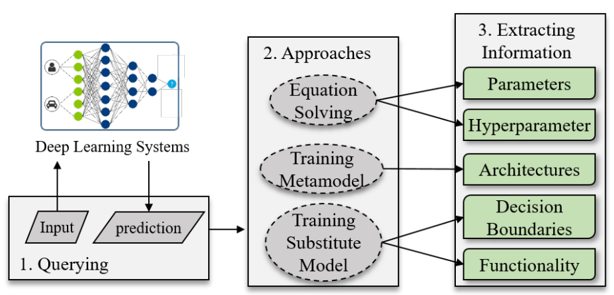
\includegraphics[scale = 0.9]{Figures/figura_14.PNG}
\decoRule
\caption[ ataque de extracción]{Ejecución de un ataque de extracción de modelo \parencite{r32}.}
\label{fig:14}
\end{figure}




\section{Envenenamiento de datos [Poison attack]}

Las redes neuronales artificiales realizan la detección de patrones en base a los datos que se utilizaron en su entrenamiento. En este contexto existe un tipo de ataque llamado envenenamiento de datos o causativos \parencite{r43}, el cual puede ser ejecutado de dos formas que se detallan a continuación, ambas con la intención de provocar que el modelo no pueda clasificar correctamente los datos, ya que se intervino el proceso de aprendizaje \parencite{r34}. 

\begin{itemize}
\item Alteración de las etiquetas del conjunto de datos: En este caso el atacante tiene acceso a los datos con los que se entrenará el clasificador, y procede a modificar las etiquetas, con algún algoritmo o de manera aleatoria.
\item Modificación del contenido de los datos: El atacante podría alterar los datos del conjunto de datos a ser utilizado en el proceso de entrenamiento, incluso de manera imperceptible a una revisión humana. 
\end{itemize}

El ataque podría no querer afectar la eficacia del clasificador excepto para un tipo de patrón determinado en el cual el atacante lograría conducir una respuesta errónea específica (técnica conocida como creación de puerta trasera). Cuando se utiliza un banco de datos públicos para entrenamiento de redes, estamos confiando que aquellos datos y sus etiquetas son correctas. Por otro lado, es muy difícil percibir si los datos fueron manipulados, ya que generalmente se utiliza cientos de miles de datos y etiquetas. La figura~\ref{fig:15} el flujo de operación de un envenenamiento de datos en un modelo de clasificación de imágenes.

\begin{figure}[th]
\centering
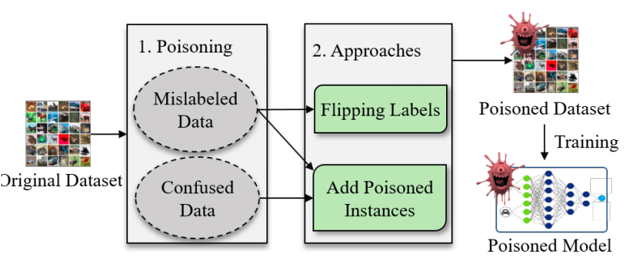
\includegraphics [scale = 0.85] {Figures/figura_15.PNG}
\decoRule
\caption[Envenenamiento de datos]{Envenenamiento de datos, flujo de operación \parencite{r32}
.}
\label{fig:15}
\end{figure}



\section{Ataques adversarios [Adversarial attack]}

Se han realizado estudios respecto a las diferencias entre el razonamiento humano versus el de las redes neuronales para clasificar imágenes, en donde se crean imágenes que no tienen ningún sentido para una persona, pero un clasificador lo identifica con un porcentaje de confidencialidad de hasta un 99,9\% \parencite{r10}. La figura~\ref{fig:16} muestra las imágenes creadas usando algoritmo evolutivo, en donde un clasificador interpreta como un número, cuando en realidad solo hay ruido. En el experimento el autor crea poblaciones iniciales (imágenes) aleatorias equivalentes a ruido, y se itera haciendo mezclas entre los individuos que obtienen mayor confidencialidad en las respuestas del clasificador, llegando a obtener imágenes que no tiene ninguna interpretación a vista de un humano, pero si para la máquina, demostrando que existen diferencias en la forma en que las redes neuronales y los humanos interpretan las imágenes, lo que explica las vulnerabilidades señaladas en adelante.

\begin{figure}[th]
\centering
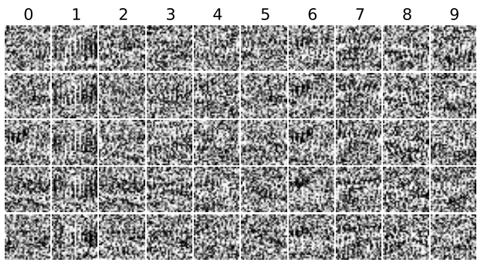
\includegraphics [scale = 0.95] {Figures/figura_16.PNG}
\decoRule
\caption[Ruido interpretado]{Ruido interpretado como números (etiqueta por columna) \parencite{r10}.}
\label{fig:16}
\end{figure}

Los ataques adversarios, también conocidos como exploratorios, son un conjunto de técnicas en la cual el atacante intenta alterar el resultado de un clasificador de un sistema de aprendizaje automático al producir una pequeña perturbación en la entrada \parencite{r4}, cuyo objetivo es que dicha entrada pueda ser clasificada correctamente por un humano, pero no así por un clasificador de inteligencia artificial. Esta perturbación puede resultar ser imperceptible al ojo humano, pero suficiente para que el clasificador arroje una salida errónea o incluso una deseada por el atacante. 

\subsection{Ataque de caja blanca}

En un ataque de caja blanca el atacante tiene acceso al modelo, por lo que además conoce la parametrización de la red como también la arquitectura. Papernote dispuso un marco de trabajo \parencite{r40} el cual permite crear ejemplos adversarios (datos manipulados para el ataque) desde el mismo modelo objetivo del ataque. Por ejemplo, un atacante podría pretender que el clasificador interprete una imagen con el número uno como un cuatro. Para ello analiza la dirección en que debe modificar la imagen resolviendo cuales píxeles de la imagen deben ser modificados. Luego selecciona el tamaño de la perturbación, generalmente buscando el mínimo necesario para lograr el objetivo. Con lo anterior ya se ha creado una nueva imagen que parece ser un número uno, pero este podría ser clasificado como cuatro por el modelo. Si el clasificador no da la respuesta deseada por el atacante, se itera en el ciclo hasta conseguirlo (por ejemplo, aumentando el tamaño de la perturbación). 
Durante el entrenamiento de una red neuronal artificial se suele utilizar la técnica de backpropagation para realizar constantes ajustes a los pesos de las conexiones de la red para obtener los resultados que minimicen la función de pérdida (errores de las clasificaciones). Estos ajustes se propagan desde la capa de salida a las capas anteriores. El gradiente descendente en este proceso de ajuste indica en qué dirección y en qué medida se debe realizar el ajuste para mejorar la clasificación. Esta técnica de aprendizaje es utilizada en forma inversa por el atacante para maximizar el error de la red frente a una entrada modificada maliciosamente, cómo se indicará a continuación. 

Las técnicas más reconocidas para la generación de ataques adversarios son las siguientes \parencite{r19}:

\subsubsection{L-BFGS}

Szegedy \parencite{r4} fue el primero en introducir el término ejemplos adversarios [adversarial example], presentando el siguiente problema de minimización para su generación:

\begin{figure}[th]
\centering
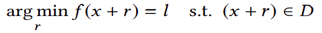
\includegraphics [scale = 0.75]{Figures/formula1.PNG}
\label{fig:f1}
\end{figure}

En la fórmula anterior “x” es el dato original de entrada a la red, “f” es la función de clasificación que representa la operación de la red la cual entrega los resultados del modelo en base a los parámetros de entrada. El ejemplo adversario está representado por “x + r”, que pertenecen al dominio “D” de la red, “l” es la etiqueta incorrecta. El autor plantea el uso del método de optimización L-BFGS para obtener el mínimo valor de “r” capaz de hacer fallar la clasificación, para lo cual hace uso de la gradiente descendiente de la función. Una desventaja de esta técnica es la gran cantidad de cómputo necesaria para obtener el mínimo.



\subsubsection{Fast gradient sign attack}

La técnica de ataque conocida como FGSM (siglas de su nombre en inglés fast gradient sign attack) \parencite{r3} es del tipo “caja blanca” aunque también suele ser efectiva en ataques de caja negra. Genera perturbaciones en la imagen de entrada de la red neuronal artificial utilizando el gradiente descendente, el mismo utilizado en el entrenamiento de la red, pero esta vez en dirección opuesta de manera de generar un nuevo dato de entrada el cual al ser clasificado por el modelo haría fallar su resultado. En el caso de clasificación de imágenes las entradas son matrices de píxeles. Al aplicar la técnica FGSM a partir de una imagen se genera una nueva, cuyos píxeles son modificados para que contribuyan a aumentar el resultado de la función de pérdida de la red, es decir en dirección opuesta a la utilizada en el back propagation para la corrección de pesos, llevando al clasificador a entregar un resultado distinto al que hubiese entregado con la imagen original, pero visualmente imperceptible a una revisión humana.
La generación de la imagen adversaria utilizando FGSM se realiza utilizando el modelo de la red a ser atacada, con la siguiente formula \parencite{r3} utilizando la función de gradiente descendiente:

\begin{figure}[th]
\centering
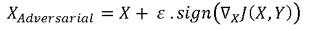
\includegraphics [scale = 0.75]{Figures/formula2.PNG}
\label{fig:f2}
\end{figure}

\begin{itemize}
    \item $\varepsilon$: Es el factor asociado al grado de la transformación. Indica el tamaño de la perturbación. Toma valores entre 0 y 1.
    \item X: Imagen original (entrada de la red neuronal artificial).
    \item Y: Etiqueta de clasificación correcta para la entrada X.
    \item J($\theta$, X, Y): Función de pérdida utilizada en el entrenamiento. Donde θ representa los parámetros del modelo. 
    \item $\bigtriangledown_x$ J($\theta$, X, Y): Gradiente descendente del clasificador.
\end{itemize}

El objetivo de FGSM es provocar que una entrada haga cruzar la frontera de decisión del clasificador hacia una respuesta incorrecta. La figura~\ref{fig:17} representa esta situación en un modelo de dos clases, en el cual una entrada correspondiente a la clasificación “círculo azul” es modificada de tal forma que el clasificador lo interpreta como “triángulo rojo”.

\begin{figure}[th]
\centering
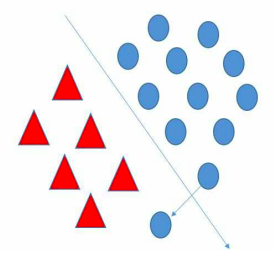
\includegraphics [scale = 0.95] {Figures/figura_17.PNG}
\decoRule
\caption[frontera de decisión]{Traspaso de frontera de decisión. Ataque FGSM \parencite{r4}.}
\label{fig:17}
\end{figure}

En la figura~\ref{fig:18} vemos un ejemplo real de cómo opera el ataque FGSM \parencite{r3}. En él vemos una entrada X que corresponde a un panda, la cual está clasificada correctamente por la red, con una exactitud del 57.7\%. Luego de utilizar el gradiente descendiente del modelo para generar una perturbación de tamaño  la cual es sumada a la imagen inicial, generando una nueva imagen que a vista humana sigue siendo un panda, pero el modelo lo clasifica como otro animal y con una exactitud del 99.3\% la cual es incluso mayor a la de la imagen original. La imagen generada es llamada ejemplo adversario [adversarial example].

\begin{figure}[th]
\centering
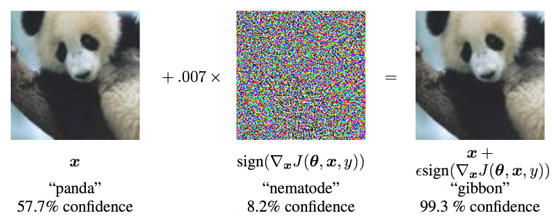
\includegraphics [scale = 0.95] {Figures/figura_18.PNG}
\decoRule
\caption[FGSM]{Ejemplo de ataque FGSM \parencite{r3}.}
\label{fig:18}
\end{figure}

La figura~\ref{fig:19} muestra un ataque a una red neuronal artificial de clasificación de imágenes de dígitos numéricos. En ella se muestra para un conjunto de datos de entrada, distintos valores de $\varepsilon$, para presentar como se ve afectada la imagen y la clasificación a medida que aumenta el tamaño de la perturbación. Un $\varepsilon$ igual a cero representa la imagen original, la cual fue correctamente clasificada. Desde $\varepsilon$ 0,05 el algoritmo clasifica mal, pero la imagen no parece haber sido manipulada. A medida que aumenta $\varepsilon$ la imagen muestra colores sospechosos para la vista humana, no así para el modelo, ya que incrementa la probabilidad de que este arroje una respuesta errónea.

\begin{figure}[th]
\centering
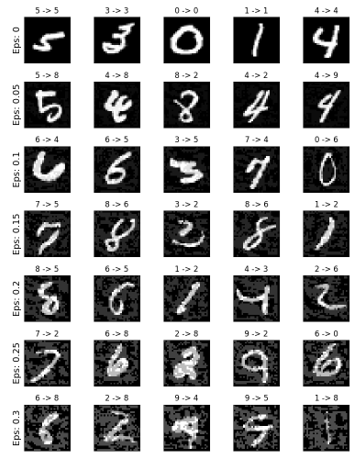
\includegraphics [scale = 1] {Figures/figura_19.PNG}
\decoRule
\caption[MNIST]{Distintos valores eps sobre MNIST \parencite{r3}.}
\label{fig:19}
\end{figure}



\subsubsection{Método de clase objetivo [Target class method]}

Este ataque puede también ser dirigido no solo para hacer fallar la clasificación, sino también para que esta clasifique en un valor deseado por el atacante. El método de clase objetivo es una variante de FGSM \parencite{r37} en el cual el atacante define la respuesta errónea que desea recibir del clasificador y busca las perturbaciones necesarias para dicho objetivo. La figura~\ref{fig:20} muestra un ejemplo de esto, en donde con una imagen del dígito 1 el atacante itera en la confección del ejemplo adversario hasta conseguir que el modelo lo clasifique con el valor 4.

\begin{figure}[th]
\centering
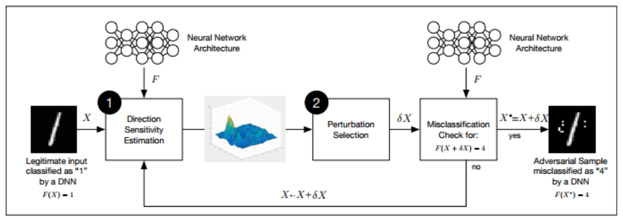
\includegraphics [scale = 0.9] {Figures/figura_20.PNG}
\decoRule
\caption[adversario dirigido]{Ejemplo adversario dirigido \parencite{r24}.}
\label{fig:20}
\end{figure}

\subsubsection{Método de clase objetivo [Método Jacobiano]}

Este método permite generar ataques dirigidos, es decir cuando el atacante desea que la red arroje un resultado específico de su interés. Papernote \parencite{r13} plantea en su investigación el uso del método Jacobiano como una forma de obtener la dirección de sensibilidad, es decir el Jacobiano de la función de aprendizaje (matriz de derivadas parciales). La construcción del ejemplo adversario en este método se realizan utilizando la matriz Jacobiana para crear el mapa de perturbaciones necesarias para obtener la salida deseada de la red. Para dirigir la salida de la red se itera observando cómo las perturbaciones en la entrada afectan la salida. El mapa de prominencias (map saliency) indica en qué píxeles de la entrada (en el caso de clasificación de imágenes) la red presenta más sensibilidad para inclinar su resultado a una clase determinada. La figura~\ref{fig:21} muestra un mapa de prominencias asociada a una imagen de 28x28 píxeles, el valor absoluto del eje Y indica que perturbaciones en la entrada obtendría mayor efectividad de llevar a la salida a un resultado deseado.

\begin{figure}[th]
\centering
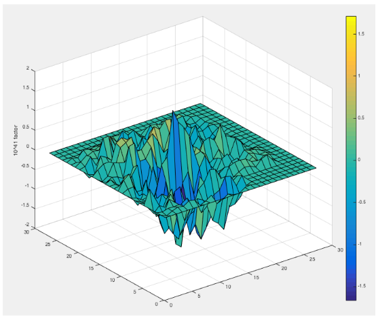
\includegraphics [scale = 1] {Figures/figura_21.PNG}
\decoRule
\caption[Mapa]{Mapa de protuberancias que indica en cuales píxeles de una imagen de 28x28 existe mayor sensibilidad en el clasificador \parencite{r13}.}
\label{fig:21}
\end{figure}

La figura~\ref{fig:22} indica resultados de estudio citado \parencite{r13}, en donde con el método Jacobiano se dirige el ataque para obtener un resultado específico en cada dígito, cuya imagen original se encuentra en la diagonal. El conjunto de datos utilizado es el MNIST de detección de dígitos. El ataque logró para cada dígito de entrada dirigirlo a cada una de las clases del clasificador. Se observa que para algunos dígitos se requiere mayor manipulación que para otros, como por ejemplo lograr que un 5 sea clasificado como un 1. Por otro lado, hay casos como el llevar al clasificar a confundir un 3 con un ocho, en donde prácticamente la perturbación es imperceptible a la vista humana. El dígito 1 resultó ser en promedio el más vulnerable de llegar a ser clasificado como cualquier otro dígito, con menores alteraciones.

\begin{figure}[th]
\centering
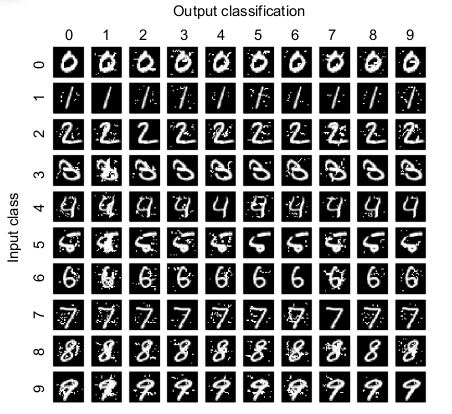
\includegraphics [scale = 1] {Figures/figura_22.PNG}
\decoRule
\caption[Mapa]{Perturbaciones dirigidas con metodo Jacobiano \parencite{r13}.}
\label{fig:22}
\end{figure}




\subsubsection{Método de clase objetivo [Ataque CW]}
Carlini y Wagner \parencite{r55} propusieron una técnica de ataque que no utiliza el gradiente descendiente de un modelo entrenado, en su lugar utiliza parámetros asociados a una regresión del clasificador. Ellos experimentaron con diferentes formulaciones de la función objetivo de la optimización para encontrar ejemplos adversarios en ataques de caja blanca. Descubrieron que minimizar una suma ponderada de la norma de perturbación y una función de pérdida de clasificación particular, Losscw, ayuda a lograr ataques más imperceptibles. Definieron la función Losscw no directamente sobre las probabilidades emitidas por clasificador, sino sobre los logits. Este se define como el logaritmo neperiano (log) del cociente de probabilidades de dos sucesos. En términos generales, Losscw se define de la siguiente manera: 

\begin{figure}[th]
\centering
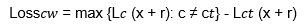
\includegraphics [scale = 0.75]{Figures/formula3.PNG}
\label{fig:f3}
\end{figure}

Donde Lc (·) es el logit para la clase c. Maximizar la función de pérdida ($Loss_{c_w}$) aumenta la probabilidad de la clase objetivo, ct, y disminuye la probabilidad de otras.




\subsubsection{AGN redes generativas adversarias}

Un estudio reciente \parencite{r56} propone entrenar una GAN (redes neuronales generativas) que toma una imagen como entrada y genera una versión perturbada de la misma imagen que estaría mal clasificada para crear imágenes perturbadas por el adversario que conducen a una clasificación errónea. Estos ataques solo requieren que las perturbaciones tengan una pequeña norma y permitan que las perturbaciones cubran solo una pequeña porción específica de la imagen y múltiples objetivos (por ejemplo, generar anteojos que conduzcan a una clasificación errónea y parezcan realistas). 
Las GAN proporcionan un marco de trabajo para entrenar una red neuronal, denominada generador (G), para generar datos que pertenecen a una distribución (cercana a la real). G mapea muestras de una distribución Z de vectores d-dimensionales de reales entre -1 y 1 a muestras de la distribución objetivo. Para entrenar a G, se usa otra red neuronal, llamada discriminador (D). El objetivo de D es discriminar entre muestras reales y generadas. Por lo tanto, el entrenamiento puede conceptualizarse como un juego con dos jugadores, D y G, en el que D está entrenado para emitir 1 en ejemplos reales y 0 en muestras generadas, y G está entrenado para generar salidas que son (mal) clasificadas como reales por D. En la práctica, el entrenamiento se desarrolla de forma iterativa y alterna entre la actualización de los parámetros de G y D mediante backpropagation.

\subsection{Ataques de caja negra}

A diferencia del ataque del tipo caja blanca, en donde el atacante tiene acceso al modelo, lo que le facilita su objetivo, en los ataques de caja negra el atacante sólo tiene acceso a introducir una entrada a la red y a obtener la clasificación realizada por el modelo. A pesar de esta dificultad, estudios \parencite{r4} han demostrado que las redes neuronales artificiales son vulnerables a los ejemplos adversarios generados en modelos distintos, pero con mismas clases de salida. Esto quiere decir que el atacante puede crear un modelo propio de clasificación llamado “modelo sustituto”, y con este crear los ejemplos adversarios que usará para hacer fallar la clasificación de la red neuronal a ser atacada. La creación de los ejemplos adversarios se realizan con el gradiente descendiente tal como las técnicas de caja blanca. Esta propiedad de los modelos se le llama “transferibilidad”. Estos ataques suelen ser algo menos efectivos que en los de caja blanca, ya que en el caso de los ataques de caja negra existe una probabilidad alta en la que el ejemplo adversario no surja el efecto deseado por el atacante, dependiendo del modelo de origen, modelo destino, datos de entrenamiento. Cuando la red neuronal maliciosa es entrenada con los mismos datos con la que fue entrenada la red inicial la probabilidad que esta obtenga fronteras de clasificación similar a la red neuronal original es más alta, haciendo más efectivo el ataque. Sin embargo, si no se cuenta con estos datos, se puede usar el modelo original como caja negra para etiquetar imágenes de ejemplo o sintéticas y con estos datos entrenar el modelo sustituto. El atacante buscando mejorar su resultado podría crear varios modelos sustitutos distintos donde probar sus ejemplos adversarios, de modo de identificar cuáles de estos generalizan mejor las fallas, seleccionando así el ejemplo adversario más efectivo para lograr su cometido. Las técnicas de ataque de caja negra son más costosas en comparación a las de caja blanca, debido a que el atacante debe crear uno o varios modelos sustitutos para generar un ejemplo adversario. 
Estudios han demostrado que esta transferibilidad de los ejemplos adversarios creados desde un modelo sustituto también son efectivo en otros tipos de técnicas de aprendizaje automático como regresión logística, máquinas de vectores de soporte (SVM), árboles de decisión y K vecinos más cercanos (KNN) \parencite{r9}.




\subsection{Ataques en el mundo real}

Los ataques adversarios no solo son ejecutables de manera digital, estudios \parencite{r51, r52, r54, r56} han demostrado que es posible que surtan efecto en el mundo físico, aunque los métodos estándar para generar ejemplos de adversarios para redes neuronales no engañan constantemente a los clasificadores de redes neuronales en el mundo físico debido a una combinación de cambios como los puntos de vista, ruido de cámara y otras transformaciones naturales, lo que impone un desafío adicional que dificulta su aplicación en sistemas del mundo real \parencite{r52}.

\subsubsection{Imágenes impresas}

Una Investigación realizada en el 2018 realizó pruebas con imágenes ejemplos adversarios impresas. Se utilizó una cámara de un teléfono móvil, cuyas imágenes capturadas alimentaban la entrada de un modelo de red de aprendizaje profundo. Se utilizó impresiones (fotografías) de imágenes originales, como también de ejemplos adversarios, y se pudo observar como el clasificador en una gran fracción de los casos fue vulnerado. También se demostró que los ataques de tipo caja negra son efectivos en este contexto. La figura~\ref{fig:23} muestra uno de los experimentos en donde se tomó una imagen del conjunto de datos, la cual una vez impresa la original es correctamente clasificada por el modelo a través de la cámara del teléfono móvil (fotografía izquierda). Luego se imprimen los ejemplos adversarios, y son clasificados erróneamente por el modelo.

\begin{figure}[th]
\centering
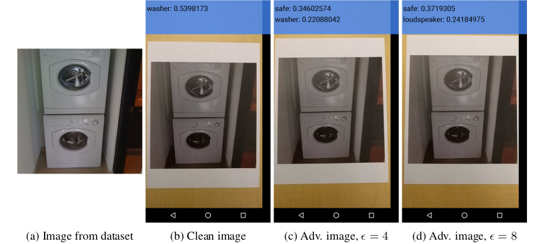
\includegraphics [scale = 1] {Figures/figura_23.PNG}
\decoRule
\caption[Mundo físico]{Ejemplos adversarios en el mundo físico. imágenes impresas \parencite{r51}.}
\label{fig:23}
\end{figure}

\subsubsection{Objetos 3D}

Estudios han realizado ataques generando ejemplos adversarios en formato 3D usando impresoras de dicha tecnología \parencite{r52} logrando hacer fallar la clasificación de un modelo de aprendizaje profundo. La figura~\ref{fig:24} muestra los objetos creados, son esculturas de tortugas, las cuales un hacen fallar la clasificación en un modelo de aprendizaje profundo. La primera fila son impresiones 3D originales. El autor implementa un tipo de algoritmo que permite, a partir de las técnicas de ataques antes mencionadas, crear ejemplos adversarios en 3D, técnica que llamó Expectation Over Transformation (EOT).

\begin{figure}[th]
\centering
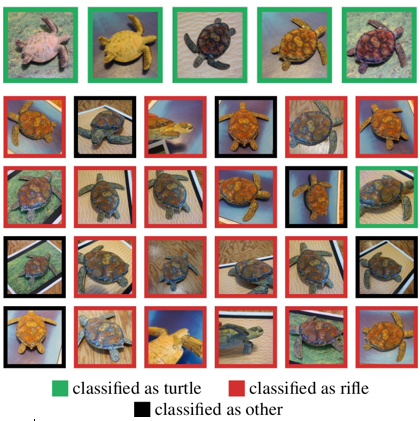
\includegraphics [scale = 1] {Figures/figura_24.PNG}
\decoRule
\caption[Ejemplos adversarios en el mundo físico. Impresión 3D]{Ejemplos adversarios en el mundo físico. Impresión 3D \parencite{r52}.}
\label{fig:24}
\end{figure}

\subsubsection{Señaléticas de tránsito}

Existen investigaciones asociadas a señaléticas de tránsito, en donde una red de aprendizaje profundo de visión artificial de un sistema de conducción automática de coches es sometida a señaléticas que han sido alteradas con parches blancos y negros logrando hacer fallar su clasificación en un 100\% en imágenes y 84.8\% en cuadros capturados por un video en un coche en movimiento,  llevando al sistema a interpretar una señalética pare como una de límite de velocidad 45 \parencite{r54}. Para lograr estas perturbaciones se utiliza una técnica de ataque llamada por el autor como “Perturbaciones físicas robustas” [Robust Physical Perturbations], que permite generar ejemplos adversarios bajo diferentes condiciones físicas. La figura~\ref{fig:25} presenta el resultado de una de las señaléticas creadas (imagen de la derecha) y se compara con una señalética que ha sido pintada con un grafiti, para evidenciar que una modificación como estas suele ser desatendidas por los conductores.

\begin{figure}[th]
\centering
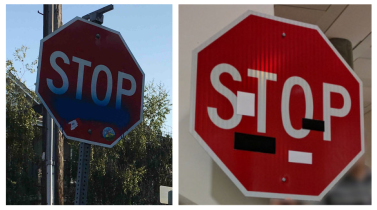
\includegraphics [scale = 1] {Figures/figura_25.PNG}
\decoRule
\caption[Ejemplos adversarios en el mundo físico. Señalética de vehículos]{Ejemplos adversarios en el mundo físico. Señalética de vehículos \parencite{r54}.}
\label{fig:25}
\end{figure}

\subsubsection{Evasión de detección facial}

Estudios realizados el año 2019 \parencite{r56} han logrado crear gafas imprimibles con un diseño y colores tal que permiten a un individuo evadir los sistemas de detección facial. Este accesorio fue diseñado utilizando un método similar a las redes generativas con adversario (GAN) con el que se entrenó una red generadora la cual crea ejemplos adversarios dirigidos, es decir que el clasificador entrega un resultado erróneo deseado por el atacante. Se toma como entrada un conjunto de imágenes de gafas. La figura~\ref{fig:26} muestra a la izquierda las gafas resultantes, que permitirían a una persona evadir la detección facial. A la derecha las imágenes originales del conjunto de datos.

\begin{figure}[th]
\centering

\includegraphics [scale = 0.9] {Figures/figura_26.PNG}
\decoRule
\caption[Ejemplos adversarios de gafas]{Ejemplos adversarios en el mundo físico. Izquierda: ejemplos adversarios de gafas. Derecha: gafas originales del conjunto de datos \parencite{r56}.}
\label{fig:26}
\end{figure}

Con la imagen de gafas del tipo ejemplo adversario se prueba la detección facial (conjunto de datos PubFig) como se muestra en la figura~\ref{fig:27}, a la izquierda la imagen original que fue reconocida por la red de aprendizaje profundo (VGG143) con probabilidad 100\%, mientras que la imagen derecha que posee los lentes adversarios (montaje digital) reconoció la persona con probabilidad menor al 0.01\%. 

\begin{figure}[th]
\centering
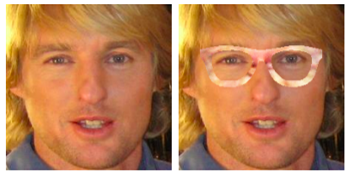
\includegraphics [scale = 1] {Figures/figura_27.PNG}
\decoRule
\caption[Imagen del actor Owen Wilson, montaje gafas de evasión de detección facial]{Ejemplos adversarios en el mundo físico. Imagen del actor Owen Wilson, montaje gafas de evasión de detección facial \parencite{r56}.}
\label{fig:27}
\end{figure}

Para implementar el ataque a nivel físico, los lentes fueron impresos y probados en personas como lo muestra la figura~\ref{fig:28}. En este experimento se logró que la persona situada en la fila superior suplante la identidad de la persona ubicada inmediatamente bajo ella.

\begin{figure}[th]
\centering
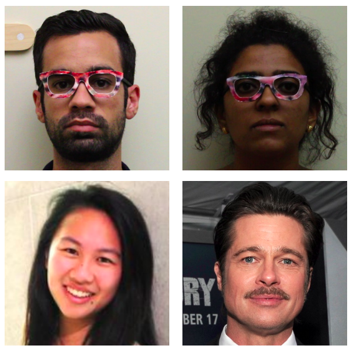
\includegraphics [scale = 1] {Figures/figura_28.PNG}
\decoRule
\caption[Suplantación de identidad]{Ejemplos adversarios en el mundo físico. Suplantación de identidad \parencite{r56}.}
\label{fig:28}
\end{figure}

\subsection{Ataques adversarios en la actualidad}
\subsubsection{Febrero 2020: Mcafee y ataque a señalética de tránsito}
La empresa Mcafee posee un área de investigación llamada Mcafee-labs, la cual recientemente liberó un artículo \parencite{r53} de una investigación asociada a la manipulación de señalética de tránsito para provocar fallos en los sistemas ADAS (Advanced Driver Assist Systems) de conducción automática utilizados por cerca de 40 millones de vehículos, incluidos los coches Tesla, con el fin de poner en discusión la seguridad de los sistemas de inteligencia artificial. Continuaron con los estudios realizados en una investigación de otro grupo de científicos \parencite{r52} que crearon un ejemplo adversario físico de una señalética pare. El equipo luego de 18 meses de trabajo logró crear señaléticas de velocidad máxima que son interpretadas erróneamente por los sistemas ADAS por una velocidad máxima mayor. 
La figura~\ref{fig:29} muestra una las imágenes resultantes. El clasificador de ADAS identifica esta señalética como una de velocidad máxima de 85 en lugar de 35. La figura~\ref{fig:30} es una fotografía del hardware de dicho sistema, el cual se utilizó en los experimentos de Mcafee. 

\begin{figure}[th]
\centering
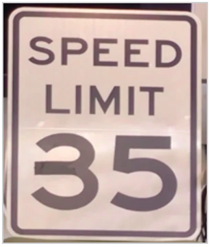
\includegraphics [scale = 1] {Figures/figura_29.PNG}
\decoRule
\caption[Ejemplo adversario de imagen de límite de velocidad]{Ejemplo adversario de imagen de límite de velocidad interpretado como velocidad máxima 85 \parencite{r53}.}
\label{fig:29}
\end{figure}

\begin{figure}[th]
\centering
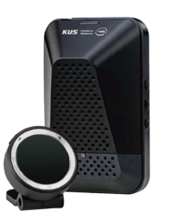
\includegraphics [scale = 1] {Figures/figura_30.PNG}
\decoRule
\caption[Hardware de sistema ADAS (Advanced Driver Assist Systems) ]{Hardware de sistema ADAS (Advanced Driver Assist Systems) \parencite{r53}.}
\label{fig:30}
\end{figure}
Lo expuesto es una señal de precaución para los conductores de vehículos autónomos ya que muchos conductores sobreestiman esta tecnología.




\subsubsection{Junio 2020: Caso Burger King}
Recientes noticias \parencite{r57} relatan una situación vivida por usuarios de vehículos de conducción automática Tesla, los cuales ante una señal vertical con el logo de Burger King provocaba que el vehículo se detuviera, ya que interpretaba la imagen como un signo pare. No hay antecedentes sobre si el anuncio publicitario fue preparado para provocar la detención de los vehículos, pero lo ocurrido demuestra lo distinto que funciona la interpretación de los sistemas de aprendizaje automático y la vista humana. Afortunadamente esta situación no provocó accidentes, pero dejó en evidencia que esta tecnología no está completamente desarrollada. La noticia se viralizó en Norteamérica y ante esto Burger King publicó en sus redes sociales “La inteligencia artificial sabe lo que anhelas”.
Es importante saber que la automatización de estos vehículos se considera en el Nivel 2 de automatización de las capacidades de conducción, lo que significa que es de un tipo asistida por el conductor y no completamente autónoma.

\begin{figure}[th]
\centering
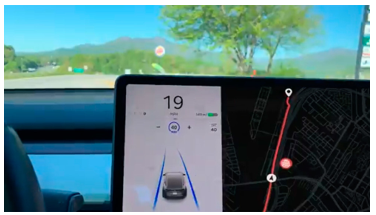
\includegraphics [scale = 1] {Figures/figura_31.PNG}
\decoRule
\caption[Vehículo de conducción automática confunde una publicidad con signo pare]{Vehículo de conducción automática confunde una publicidad con signo pare \parencite{r57}.}
\label{fig:31}
\end{figure}